
\chapter{Segmentation}

Segmentation of medical images is a challenging task. A myriad of
different methods have been proposed and implemented in recent
years. In spite of the huge effort invested in this problem, there is
no single approach that could generally solve the problem of
segmentation for the large variety of image modalities existing today.

The most effective segmentation algorithms are obtained by carefully
customizing combinations of components. The parameters of these components are
tuned for the characteristics of the image modality used as input and the
features of the anatomical structure to be segmented. 

The Insight toolkit provides a basic set of algorithms that can be used to
develop and customize a full segmentation application. Some of the most
commonly used segmentation components are described in the following sections.


\section{Region Growing}

Region growing algorithms have proven to be a very effective approach for image
segmentation. The basic concept of a region growing algorithm is to start from
a seed region that is considered to belong to the object to be segmented. The
pixels neigboring this initial region are evaluated to determine if they could
also be considered part of the object, in which case they are added to the
region. When some of the neighbor pixels are included in the region, other
pixels become new neighbors and hence become candidates to be evaluated and
eventually included in the region. Region growing algorithms vary depending on
the criteria used to decide whether a pixel should be included in the region
or not, the type of neighbor connectivity used on the image grid and the
strategy used for visiting the neighbor pixels.

Several implementations of region growing are available in the
Insight toolkit. This section describes some of the most commonly used.

\subsection{Connected Threshold}

The simplest criterion for including pixels in a growing region is
probably the condition of having intensity values inside a specific
interval.

\label{sec:ConnectedThreshold}
\ifitkFullVersion 
\input{ConnectedThresholdImageFilter.tex}
\fi


\subsection{Neighborhood Connected}
\label{sec:NeighborhoodConnectedImageFilter}
\ifitkFullVersion 
\input{NeighborhoodConnectedImageFilter.tex}
\fi



\subsection{Confidence Connected}
\label{sec:ConfidenceConnected}
\ifitkFullVersion 
\input{ConfidenceConnected.tex}
\fi


\subsection{Isolated Connected}
\label{sec:IsolatedConnected}
\ifitkFullVersion 
\input{IsolatedConnectedImageFilter.tex}
\fi


\section{Segmentation Based on Watersheds}
\label{sec:WatershedSegmentation}
\ifitkFullVersion 
\input WatershedSegmentation.tex
\fi


\section{Level Sets Segmentation}
\label{sec:LevelSetsSegmentation}
\ifitkFullVersion 
%%%%%%%%%%%%%%%%%%%%%%%%%%%%%%%%%%%%%%%%%%%%%%%%%%%%%%%%%%%%%%%%%%%%%%%%
%
%
%     This file is included from the file   Segmentation.tex
% 
%     Section tag and label are placed in this top file.
%
%
%
%%%%%%%%%%%%%%%%%%%%%%%%%%%%%%%%%%%%%%%%%%%%%%%%%%%%%%%%%%%%%%%%%%%%%%%%



\subsection{Threshold Level Set Segmentation}

\subsection{Fast Marching Segmentation}

\subsection{Shape Detection Segmentation}

\subsection{Geodesic Contours Segmentation}



\subsection{Segmentation Level Set Image Filter}
\label{sec:SegmentationLevelSetImageFilter}



\fi


\section{Hybrid Methods} 
\label{sec:HybridSegmentationMethods}

\ifitkFullVersion 
%%%%%%%%%%%%%%%%%%%%%%%%%%%%%%%%%%%%%%%%%%%%%%%%%%%%%%%%%%%%%%%%%%%%%%%%
%
%
%     This file is included from the file   Segmentation.tex
% 
%     Section tag and label are placed in this top file.
%
%
%
%%%%%%%%%%%%%%%%%%%%%%%%%%%%%%%%%%%%%%%%%%%%%%%%%%%%%%%%%%%%%%%%%%%%%%%%

\subsection{Introduction}
\label{sec:HybridSegmentationIntroduction}


It is sometimes convenient to combine several segmentation strategies with the
aim of taking advantage of their qualities an compensate their vulnerabilities.
The synergy between fundamentally different methodologies tends to result in
robustness and higher segmentation quality.  This section illustrates an hybrid
approach for segmentation in which two different strategies are configured to
work together. In this case, an input image is first processed by a filter
based on the concept of region growing. The criterion of acceptance in the
region is defined by a similarity measure that evaluates how homogeneous is the
path between to pixels. The output of this filter is used as a prior for
another filter that performs a full partition of the image space and then work
joining and splitting regions in order to optimize an homogeneity measure.
Details on the concepts behind those methods have been discussed in the
litterature
\cite{Angelini2002,Udupa2002,Jin2002,Imielinska2001,Imielinska2000a,Imielinska2000b}



\subsection{Background}
\label{sec:HybridSegmentationBackground}




%%%%%%%%%%%%%%%%%%%%%%%%%%%%%%%%%%%%%%%%%%%%%%%%%%%%%%%%%%%%%%%%%
%
%  Here is an example of how to include diagram in a figure
%
%  The file HybridSegmentationDiagram1.fig should be in the "Art"
%  directory. CMake will convert it to EPS before running latex. 
%
%%%%%%%%%%%%%%%%%%%%%%%%%%%%%%%%%%%%%%%%%%%%%%%%%%%%%%%%%%%%%%%%%

\begin{figure}
\center
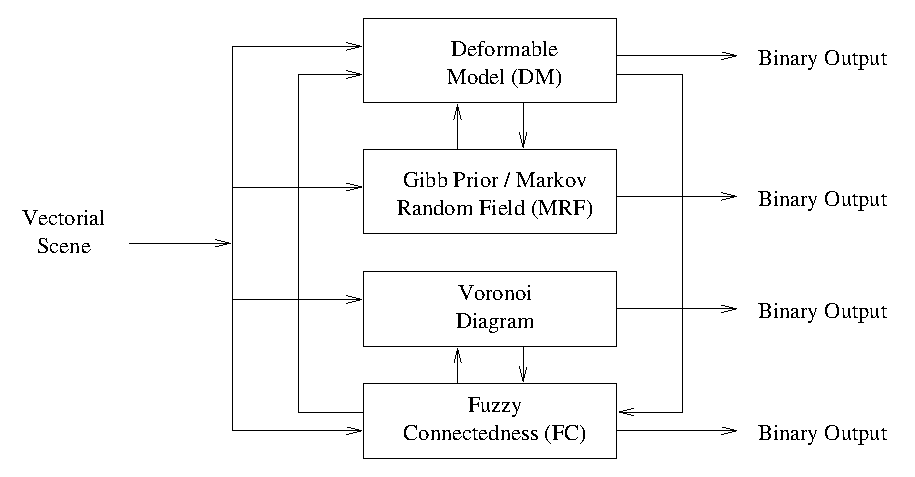
\includegraphics[width=6cm]{HybridSegmentationEngine1.eps}
\caption{Components of a HybridSegmentation approach}
\label{fig:HybridSegmentationEngine1}
\end{figure}

The Figure \ref{fig:HybridSegmentationEngine1} illustrates the main
components of the hybrid segmentation algorithm.

\begin{figure}
\center
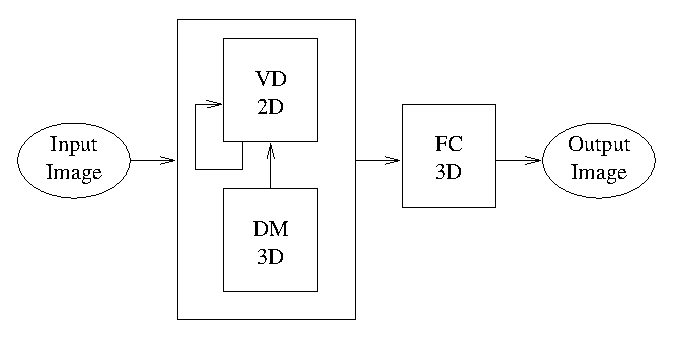
\includegraphics[width=6cm]{HybridSegmentationFCVDDM.eps}
\caption{Components of a HybridSegmentation approach}
\label{fig:HybridSegmentationFCVDDM}
\end{figure}


\begin{figure}
\center
\includegraphics[width=6cm]{VoronoiSegmentationClassDiagram1.eps}
\caption{UML Class Diagram of the VoronoiSegmentation filter}
\label{fig:VoronoiSegmentationClassDiagram1}
\end{figure}


\begin{figure}
\center
\includegraphics[width=6cm]{FuzzyConnectednessClassDiagram1.eps}
\caption{UML Class Diagram of the FuzzyConnectedness filter}
\label{fig:FuzzyConnectednessClassDiagram1}
\end{figure}


\begin{figure}
\center
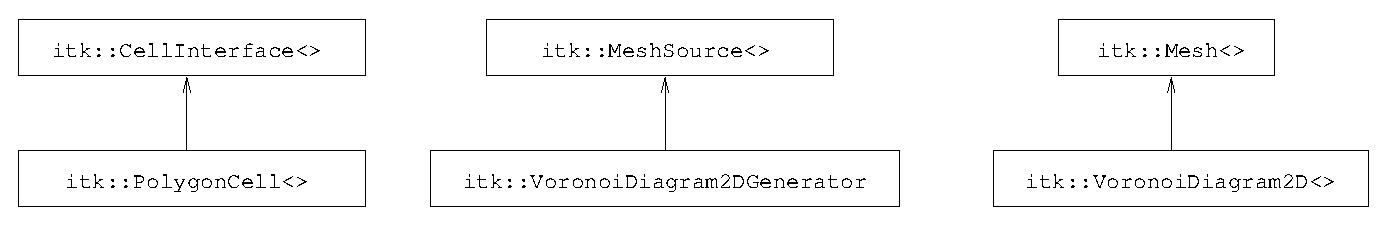
\includegraphics[width=6cm]{VoronoiSegmentationCollaborationDiagram1.eps}
\caption{UML Collaboration Diagram of the VoronoiSegmentation filter}
\label{fig:VoronoiSegmentationCollaborationDiagram1}
\end{figure}



\begin{figure}
\center
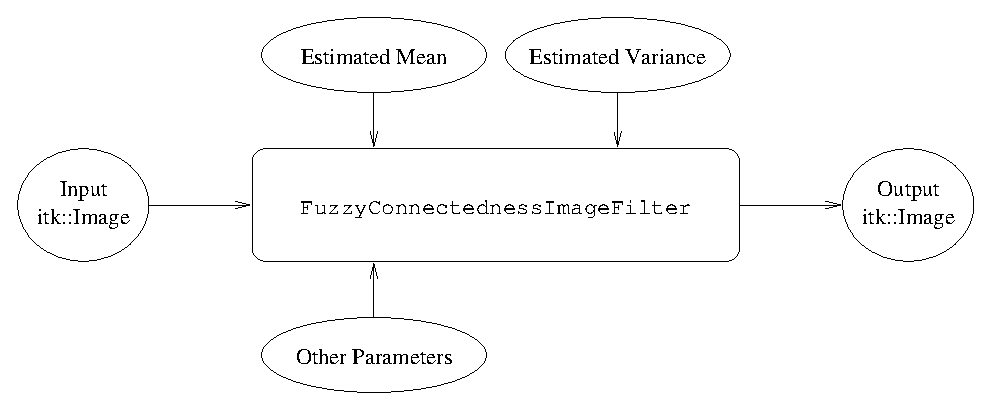
\includegraphics[width=6cm]{FuzzyConnectednessCollaborationDiagram1.eps}
\caption{UML Collaboration Diagram of the FuzzyConnectedness filter}
\label{fig:FuzzyConnectednessCollaborationDiagram1}
\end{figure}



\begin{figure}
\center
\includegraphics[width=6cm]{VoronoiSegmentationCollaborationDiagram2.eps}
\caption{UML Collaboration Diagram of the VoronoiSegmentation filter}
\label{fig:VoronoiSegmentationCollaborationDiagram2}
\end{figure}




\begin{figure}
\center
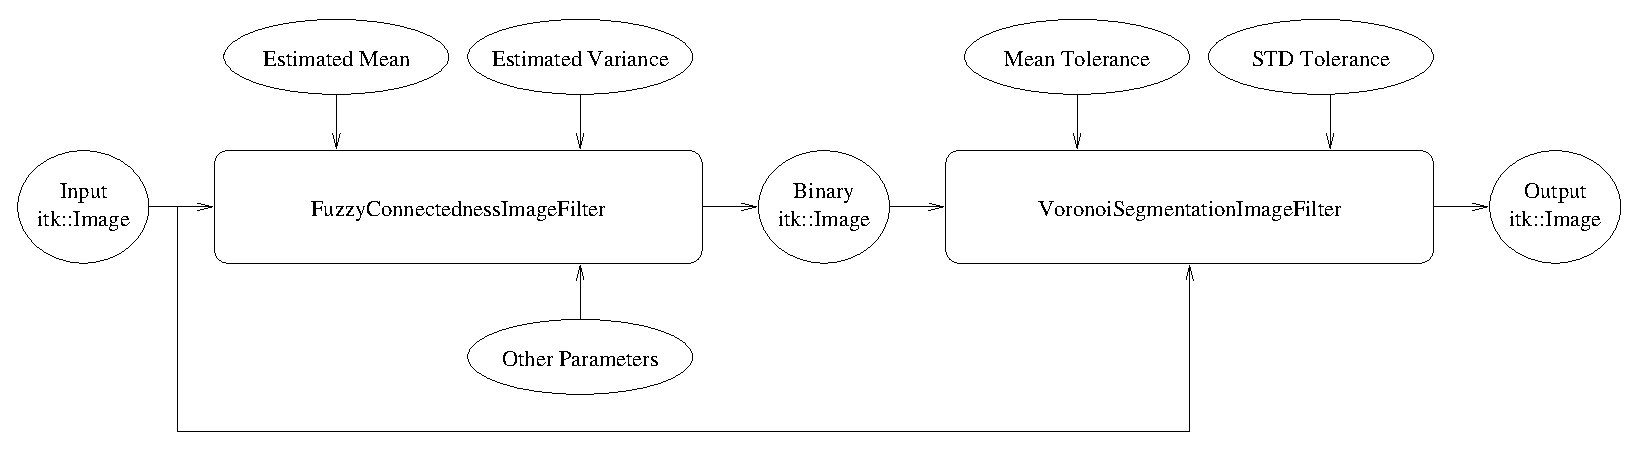
\includegraphics[width=6cm]{FuzzyVoronoiCollaborationDiagram1.eps}
\caption{UML Collaboration Diagram of the Fuzzy Voronoi Segmentation}
\label{fig:FuzzyVoronoiCollaborationDiagram1}
\end{figure}




\begin{figure}
\center
\includegraphics[width=6cm]{FuzzyVoronoiDeformableCollaborationDiagram1.eps}
\caption{UML Collaboration Diagram of the Fuzzy Voronoi Deformable Segmentation}
\label{fig:FuzzyVoronoiDeformableCollaborationDiagram1}
\end{figure}









%%%%%%%%%%%%%%%%%%%%%%%%%%%%%%%%%%%%%%%%%%%%%%%%%%%%%%%%%%%%%%%%%
%
%  Here is an example of how to include equations
%
%%%%%%%%%%%%%%%%%%%%%%%%%%%%%%%%%%%%%%%%%%%%%%%%%%%%%%%%%%%%%%%%%


\begin{equation}
MS(A,B) = \frac{1}{N} \sum_i^N \left( A_i - B_i \right)^2
\end{equation}





\subsection{Example}
\label{sec:HybridSegmentationExample1}

\input{HybridSegmentationFuzzyVoronoi.tex}



\fi


